\input{preamble.tex}
\usetikzlibrary {datavisualization}

\newcommand{\tableaucroise}[4]{
\begin{tabular}{|c|c|c|c|}
	\cline{2-4}
	\multicolumn{1}{c|}{} & #1 \\ \hline
	#2 \\ \hline
	#3  \\ \hline
	#4  \\ \hline
\end{tabular}
}

\begin{document}

\reversemarginpar

\pagestyle{fancy}
\fancyhead[L]{Terminale STMG}
\fancyhead[C]{\textbf{Préparation DS n°7 (probabilités)}}
\fancyhead[R]{\today}

\null\vspace{-30pt}
Nom / Prénom : \\

Consignes particulières : 
\begin{itemize}[label=$\bullet$]
	\item 
	La calculatrice est {autorisée}.
	\item 
	L'exercice \ref{exe:1} peut être fait partiellement sur la feuille.
	\item 
	Ce devoir \textbf{n'est pas noté} il a vocation à vous préparer.
\end{itemize}

\hrule

\exe{}{
On donne l'arbre ci-dessous :
\begin{center}
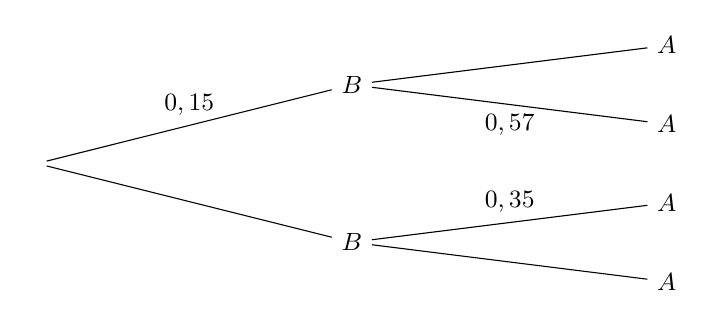
\begin{tikzpicture}[scale=1]
\node {}[grow=right, level distance=4cm, sibling distance=2cm]
	child {node {\small $\widebar{B}$}[level distance=4cm, sibling distance=1cm]
		child {node{\small $\widebar{A}$}
		}
		child {node{\small $A$}
			edge from parent node[above] {\small $0,35$}
		}
	}
	child {node {\small $B$}[level distance=4cm, sibling distance=1cm]
		child {node{\small $\widebar{A}$}
			edge from parent node[below] {\small $0,57$}
		}
		child {node{\small $A$}
		}
		edge from parent node[above] {\small $0,15$}
	}
;
\end{tikzpicture}
\end{center}
Calculer (arrondir si nécessaire) :
\begin{multicols}{3}
\begin{enumerate}
\item $P(\widebar{B})$
\item $P_B(A)$
\item $P_{\widebar{B}}(\widebar{A})$
\item $P(A \cap B)$
\item $P(A \cap \widebar{B})$
\item $P(\widebar{A} \cap \widebar{B})$
\item $P(A)$
\item $P(\widebar{A})$
\item $P_A(B)$
\item $P_{\widebar{A}}(B)$
\item $P_A(\widebar{B})$
\item $P_{\widebar{A}}(\widebar{B})$
\end{enumerate}
\end{multicols}
}{exe:1}{
Voir cours.
}

\exe{}{
On lance une pièce déséquilibrée (c'est-à-dire dont on ne connaît pas la probabilité de tomber sur pile ou face).
On note $p$ la probabilité que le pièce tombe sur pile.
Lorsque la pièce tombe sur pile, on tire une boule dans une urne contenant 4 boules vertes et 6 boules rouges. \\
Lorsque la pièce tombe sur face, on tire une boule dans une seconde urne contenant 8 boules vertes et 2 boules rouges. \\
On note $R$ l'évènement \og tirer une boule rouge \fg.
\begin{enumerate}
\item Montrer que la probabilité de tirer une boule rouge est donnée par $P(R) = 0,2 + 0,4p$.
\item Estimer $p$ si les probabilités de tirer une boule verte ou rouge sont égales.
\item Est-ce possible que $P(R)=0,1$ ? Justifier.
\item On constate que $P(R)=0,28$. Estimer le nombre de piles obtenus en réalisant 5 lancers de pièces.
\end{enumerate}
}{exe:2}{
\begin{enumerate}
\item En réalisant un arbre de probabilité, on trouve $P(R) = 0,6p + 0,2(1-p) = 0,2 + 0,4p$. 
\item Si $P(R)=P(V)=0,5$ alors on résout $0,5 = 0,2 + 0,4p$ soit $p=0,75$.
\item Dans ce cas on trouve $0,1=0,2+0,4p$ soit $p=-0,25$ ce qui est impossible.
\item Toujours en résolvant, on trouve $p=0,2=\dfrac15$ soit, en moyenne, 1 pile pour 5 lancers.
\end{enumerate}
}

\exe{}{
Un lycée comporte 2~463 élèves. 
Parmi les élèves, 880 sont en filière professionnelle, les autres sont en filière GT (générale/technologique).
Parmi les élèves en filière GT, 923 sont des filles.
Parmi les élèves en filière professionnelle, 673 sont des garçons. \\
\begin{enumerate}
\item 
Compléter le tableau croisé ci-dessous :
	\begin{center}
	%\def\arraystretch{1.8}
	\setlength\tabcolsep{20pt}
	\tableaucroise{Garçon & Fille & Total}{Pro & & &}{GT & & &}{Total &&&}
	\end{center}
Un élève du lycée est tiré aléatoirement pour recevoir un prix exceptionnel (un croissant gratuit). Calculer :
\begin{enumerate}
\item la probabilité que cet élève soit un garçon ;
\item la probabilité que cet élève soit un garçon en filière professionnelle ;
\item la probabilité que cet élève soit en filière GT sachant que c'est une fille.
\end{enumerate}
\item les évènements \og un garçon reçoit le prix \fg{} et \og un élève de filière professionnelle reçoit le prix \fg{} 
sont-ils indépendants ? Justifier.
\end{enumerate}
}{exe:3}{
\begin{enumerate}
\item
\begin{enumerate}
\item On divise l'effectif des garçons par l'effectif total.
\item On divise l'effectif des garçons en fillière professionel par l'effectif total.
\item On divise l'effectif des filles en filière GT par l'effectif total des filles.
\end{enumerate}
\item On compare $P(G)$ à $P_{\text{pro}}(G)$, si le probabilités sont différentes alors les évènements ne sont pas indépendants.
\end{enumerate}
}

% cf manuel
\exe{}{
Pendant les vacances d'hiver, un magasin de sport propose du matériel de ski à la location.
La moitié des locations de la journée ont été des snowboards $(S)$, 
40 \% des skis alpins $(A)$ et le reste des skis de fond $(F)$. 
Après la journée de location, le matériel est contrôlé et éventuellement réparé $(R)$. 
L'arbre pondéré représentant cette situation est donné ci-dessous :

\begin{center}
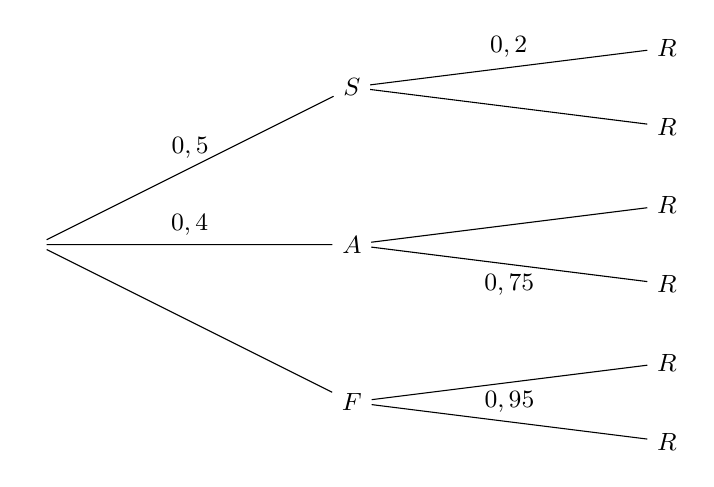
\begin{tikzpicture}[scale=1]
\node {}[grow=right, level distance=4cm, sibling distance=2cm]
	child {node {\small $F$}[level distance=4cm, sibling distance=1cm]
		child {node{\small $\widebar{R}$}
			edge from parent node[above] {\small $0,95$}
		}
		child {node{\small $R$}
		}
	}
	child {node {\small $A$}[level distance=4cm, sibling distance=1cm]
		child {node{\small $\widebar{R}$}
			edge from parent node[below] {\small $0,75$}
		}
		child {node{\small $R$}
		}
		edge from parent node[above] {\small $0,4$}
	}
	child {node {\small $S$}[level distance=4cm, sibling distance=1cm]
		child {node{\small $\widebar{R}$}
		}
		child {node{\small $R$}
			edge from parent node[above] {\small $0,2$}
		}
		edge from parent node[above] {\small $0,5$}
	}
;
\end{tikzpicture}
\end{center}

\begin{enumerate}
\item Selon vous, quels sont les utilisateurs les plus soigneux du matériel ? Justifier.
\item Quelle est la probabilité que le matériel restitué nécessite des réparations ?
\item Estimer la probabilité qu'un matériel loué soit des skis alpins sachant qu'il nécessite des réparations.
\end{enumerate}
}{exe:4}{
\begin{enumerate}
\item Les utilisateurs de snowboard.
\item On calcule $P(R) = 0,5 \times 0,2 + 0,4 \times 0,25 + 0,1 \times 0,95$.
\item On utilise la formule de Bayes pour calculer :
\[ P_R(A) = \dfrac{P(A)}{P(R)} P_A(R) . \]
\end{enumerate}
}



%%%%%%%%%%%%

\newpage
\fancyhead[C]{\textbf{Solutions}}
\shipoutAnswer


\end{document}
